\section{Methodology}
To study the effect of \acf{LOC}, we designed a Pacman game that periodically
reduced the amount of control the user has over his avatar.
The \ac{EEG} was passively recorded during game play, and afterwards the
off-line performance of an \ac{ERD} and an \ac{ERP} based classifier was used to
assess the influence of \ac{LOC} on the \ac{BCI} performance. In the rest of
this section, we describe the data collection, the preprocessing and
classification of the \ac{EEG}, and the evaluation method in more detail.

\subsection{Data collection}
%\subsubsection{The Pacman Game}\label{sec:affpac}
A game was designed to induce a state of \ac{LOC}, with game play similar to
the original Pacman game \cite{reuderink2009apf}. The major differences with
other Pacman games is that our game periodically tried to induce a state of
\ac{LOC} in the user by responding unreliably to the keyboard commands. Since
unreliable input is a proven method for frustration induction
\cite{scheirer2002fup, klein2002cru, diener2006eaa}, we expected this method to
induce mental state changes that were naturally associated with \ac{LOC}.
%
To simplify (simulated) \ac{BCI} control, the user input was reduced to a
button for the left index finger that turned Pacman 90 degrees counterclockwise,
and a button for the right index finger that turned Pacman clockwise. 

\begin{figure}
  \centering
  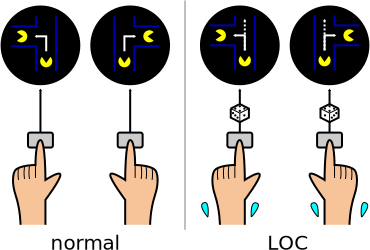
\includegraphics[width=2in]{experiment_figure}
  \caption{In the normal condition, the left button rotated the player
  $90^{\circ}$ counterclockwise; the right button rotated the player
  $90^{\circ}$ clockwise. In the \protect\ac{LOC} condition, 15\% of the
  keyboard input was ignored, and a visual lag was induced (not shown).}
  \label{fig:experiment_concept} 
\end{figure}

\subsubsection{Experiment design}
The \ac{LOC} was induced in a randomized interleaved block design with
experimental blocks of two minutes. In one third of these two-minute blocks
\ac{LOC} was induced, in the other blocks the game play remained unmodified.
The \ac{LOC} blocks were evenly distributed over the session by building a
series of shuffled sequences of three blocks (one \ac{LOC} and two normal
blocks). In the \ac{LOC} condition, the game randomly ignored 15\% of the keystrokes, resulting in a barely playable game. In addition, the display
occasionally lagged in the \ac{LOC} condition. After each block, the user was
asked to rate his mental state in terms of valence (pleasure), arousal and
dominance (subjective feelings of control) on a Likert-scale presented under
the \ac{SAM} \cite{bradly1994mes}.

\subsubsection{Experimental procedure}
Subjects were asked to read and sign a form of consent, and were subsequently
wired with the \ac{EEG} and physiological sensors. The experimenter briefly
explained the game and the self-assessment procedure. The subject was
allowed to practise the controls for two minutes before the experiment was
started. If users mentioned that the game was unresponsive during the
experiment, the experimenter asked them to continue playing and promised to
find the cause later. After 30 minutes, the experimenter stopped the experiment
and the users were debriefed.

\subsubsection{Sensors and recording}
\begin{sloppypar}
A BioSemi ActiveTwo \ac{EEG} system was used to record the \ac{EEG} and
physiological signals at a sample rate of 512~Hz. \Ac{EEG} was recorded with 32
Ag/AgCl active electrodes placed at locations of the Extended International
10-20 system. To measure the influence of ocular and muscle artifacts, we
recorded the \acs{EOG} (horizontal and vertical pairs) and two pairs of
\acs{EMG} signals over the left and right flexor digitorum profundus (the
muscles used to press with the index finger).  Additional physiological
sensors, such as temperature, respiration, the galvanic skin response and the
blood volume pulse were recorded as well, but not used in the present
study\footnote{The recordings are available at
\url{http://borisreuderink.nl/perm/affpac/}.}.
\end{sloppypar}

\subsection{Preprocessing}
The following preprocessing procedure was applied to reduce the influence of
noise and artifacts caused by eye movements and muscle tension: first the
recording was downsampled to 128 Hz to speed up processing. After downsampling,
the data was high-pass filtered using a 4th-order Butterworth filter to remove
frequencies below 0.2 Hz, and notch-filtered using a 4th-order Butterworth
filter from 49--51 Hz to remove power line noise. The \ac{EEG} was then
corrected for eye movements using a regression  based subtraction
method \cite{schloegl2007fac}.
To prevent noise from spreading to other channels, we performed
channel-level preprocessing before we applied the \ac{EOG} correction and
re-referenced the signals to the \ac{CAR}.

\subsection{Key press classification from EEG}
\begin{sloppypar}
Most motor imagery based \acp{BCI} are based on sensory-motor rhythms,
specifically the \acf{ERD} that occurs during both real and imaginary movement.
As the \ac{ERD} of real and imagined hand movement is similar
\cite{mcfarland2000mbr}, we used real movement to train \acp{BCI} that predict
the movement from the \ac{EEG} signal, since it provides a clear ground truth
and allows for a tighter controlled experiment. In this section we will outline
the classifiers used for detection of the \ac{ERD} and the \ac{ERP} associated
with the movements executed to play the game.
\end{sloppypar}

\subsubsection{\protect\ac{ERD} features}
\begin{sloppypar}
The \ac{ERD} classification was based on the decrease in the Rolandic mu rhythm
(8--12~Hz) and Rolandic beta frequencies (peak around 20~Hz) on the
contra-lateral motor cortices that occurs when movement is initiated
\cite{pfurtscheller1999eem}.
% 
After preprocessing, we applied a 6th-order Butterworth band-pass filter to
extract the frequencies from 8--30 Hz, which includes both the mu and beta
rhythms. From this filtered \ac{EEG} we extracted windows of one second,
centered on the moment that keystroke was registered. Visual inspection
confirmed that an \ac{ERD} did indeed occur within this period. For these
segments we trained subject-specific spatial filters with the \ac{CSP}
algorithm.
\end{sloppypar}

The \ac{CSP} algorithm \cite{koles1991qet} finds a matrix $\tilde{W}$ with
spatial filters that map the \ac{EEG} into a new space with basis vectors that
have a high variance for the first class and a low variance for the second, and
vice versa. Given the number of sensors $s$, and the number of samples $n$,
$W$ is an $s \times s$ transformation matrix with the following property:
%
\begin{equation}
  \Sigma_{WX_1} = D \quad \textrm{and} \quad
  \Sigma_{WX_1} + \Sigma_{WX_2} = I, 
  \label{eq:CSP_BR}
\end{equation}
%
where $D$ is a diagonal matrix with elements in descending order, $I$ is
the identity matrix and $\Sigma_{X_i}$ is the channel covariance matrix of the
$s \times n$ \ac{EEG} measurements matrix $X$ for given class $i$.
%
Rows of $W$ that correspond to a high value in $D$ have a high variance (power)
for the first class and a low variance for the second, and vice versa. Because
of this discriminatory property, the $\frac{m}{2}$ first and the $\frac{m}{2}$
last rows were picked to construct the final matrix $\tilde{W}$ with $m=6$
spatial filters.

After applying the \ac{CSP} algorithm, we calculated the variance (which
corresponded to the band power in the mu and beta band) for each transformed
channel, which resulted in $m$ spatial band-power features.

\subsubsection{\protect\acs{ERP} features}
A less frequently used paradigm for classification of \ac{EEG} related to
movement is based on the \ac{BP}, a negative \ac{ERP} related to movement
initiation. The \ac{BP} consists of an early phase beginning about 2 seconds
before the movement onset, and a late phase with a steeper slope 400~ms before
the onset \cite{shibasaki2006wb}.  We used the asymmetric distribution of the
late \ac{BP} over the scalp for classification of the laterality of the hand
movements, which is known as the \ac{LRP}.

For the \ac{ERP} classification, we used the same preprocessing pipeline as
used with the \ac{CSP} classification up to the band-pass filter. Then we
applied a (4th-order Butterworth) low-pass filter at 10~Hz, and again extracted
windows of one second centered on the moment of registration of keyboard
input. These trials were then transformed with a whitening transform $P$
which has the property that the transformed signals are uncorrelated, and have
unit variance:
%
\begin{equation} 
  \Sigma_{PX} \approx P \Sigma_X P^T = I.  
\end{equation}
%
With the eigenvalue decomposition $\Sigma_X = U \Lambda U^T$, we find that
%
\begin{equation}
  P = \Lambda^{-\frac{1}{2}} U^T. 
\end{equation}

After whitening with $P$, we downsampled the signal by taking every fourth
sample point, resulting in a $s \times \frac{e}{4}$ feature vector where
$e=128$ is the number of samples in a classification window.
%
Despite superficial differences, this method for \ac{LRP} classification is
conceptually similar to the conventional approaches for \ac{ERP} detection,
such as \cite{blankertz2003bbr, blankertz2011sta}, but does not rely on time
segment or channel picking.

\subsubsection{Classification}
The \ac{ERD} and \ac{LRP} features were used to train a final linear \ac{SVM}
classifier. The \ac{SVM}'s regularization parameter $c$ was selected with a
separate cross-validation loop on the two-minute blocks in training set. 

\subsection{Loss of control analysis} \label{sec:dga}
\begin{sloppypar}
To analyze the influence of user \ac{LOC} on the performance of a \ac{BCI},
we trained a \ac{BCI} on normal blocks, and measured the difference in
performance of the same classifier between unseen, normal blocks and unseen
blocks from the \ac{LOC} condition.
% 
As we could not assume that the distribution of the \ac{EEG} signal
would remain stationary, training and evaluating a \ac{BCI} on samples uniformly
spread over the sessions might lead to an overestimation of the performance.
In order to have a more reliable measure of how an online \ac{BCI} would
perform, we therefore used a special evaluation scheme where complete
experimental blocks were left out for evaluation:
%
The session consisted of a series of permutations of three experimental blocks;
two normal blocks, and a block with \ac{LOC} simulation. For every three
blocks, we added the first normal block to the training set for the \ac{BCI}
classifier. The remaining normal and \ac{LOC} block were used for evaluation.
This way, the training data was spread over time, but we still have independent
blocks for evaluation.
%
Note that this evaluation is not symmetrical, since the classifiers were
trained only on normal blocks, but tested on blocks of both the normal and
\ac{LOC} condition. 
\end{sloppypar}

If there were difference between the normal and \ac{LOC} conditions, we
expected to find a lower performance on \ac{LOC} blocks compared to block with
normal control, since the model was optimized for a different distribution than
the observations it was evaluated on had.

\subsection{Performance measure}
\ac{BCI} classifiers are often evaluated by comparing their accuracy on
out-of-sample trials. The choice for the accuracy measure is problematic, as
accuracies (or equivalently, error rates) are hard to interpret when the prior
probabilities of the classes are unequal and/or variable. Furthermore, the
statistic does not take the time needed to perform a trial (key press) into
account: due to our short \acp{ITI}, lower accuracies were to be expected for
our \acp{BCI} than the accuracies reported for more traditional \ac{BCI}
environments, where multiple seconds are used to detect an imagined movement.
Despite these drawbacks, we will provide accuracy measures because it is
commonly used.

\begin{sloppypar}
A more informative measure is the \ac{ITR}, which conveniently captures the
amount of information a user can communicate through a (noisy) channel with an
optimal encoding strategy. It does so by combining the quality of and the time
needed for the predictions. As such, the \ac{ITR} is a better measure to
evaluate \ac{BCI} performance.
%
Note that different formulas to calculate the \ac{ITR} are used in the \ac{BCI}
literature, for example Wolpaw's definition in \cite{wolpaw2002bci} is often
used. The drawback of this definition is that it has a number of assumptions
that are often violated in practice, most notably the assumption that all
classes have the same prior probability. The \ac{ITR} based on \ac{MI} does not
rely on these assumptions, hence we use \ac{MI} to measure the information
contained in the prediction of a single trial. Note that the labels of the
trials still need to be independent of each other for a correct estimate of the
\ac{ITR}.
\end{sloppypar}

The \Ac{MI} expresses the decrease in uncertainty of a discrete variable
$\mathcal{Y}$ (the true labels), given a discrete variable $\mathcal{Z}$ (the
predictions of the classifier):
%
\begin{equation} \label{eq:mi} I(\mathcal{Z}; \mathcal{Y}) = \sum_{\substack{y
\in \mathcal{Y}\\z \in \mathcal{Z}}} p(z, y) \log_2{\frac{p(z,
y)}{p_1(z)\,p_2(y)}}, \end{equation}
%
where $p(z, y)$ is the joint probability distribution and $p_1(z)$ and $p_2(y)$
are the marginal probability distribution functions of $\mathcal{Z}$ and
$\mathcal{Y}$. With the base-2 logarithm the reduction in uncertainty is
expressed in bits. We use the \ac{MI} between the classifiers predictions and
the ground truth as a second performance measure. The joint and marginal
probabilities in \eqref{eq:mi} were estimated by their relative frequency of
occurrence in the confusion matrix.

Finally, we calculate the third measure \ac{ITR} $R$, in bits per minute, based on the
\ac{MI} \eqref{eq:mi}, and the median\footnote{We use the median instead
of the mean because $\Delta t$ appeared to follow a Poisson distribution.} \acl{ITI} $\med(\Delta t)$:
%
\begin{equation}
  R = 60 \frac{I}{\med(\Delta t)}.
\end{equation}

As a fourth, and last performance measure, we use the \ac{AUC} of the \ac{ROC}
\cite{fawcett2005ira} to express the ranking performance of the classifier. The
\ac{AUC} is equal to the probability that a randomly chosen instance of the
first class is ranked above a randomly chosen instance of the second class;
in other words, an \ac{AUC} of 0.5 indicates random performance, and an
\ac{AUC} of 0 or 1 indicates perfect ranking ability. Like the \ac{MI}, the
\ac{AUC} does not assume equal prior probabilities.

Originally we planned to use the \ac{KLD} as a measure of change in the feature
distributions as in \cite{shenoy2006tac}, but the assumption that the features
are normally distributed was violated heavily by both our \ac{ERD} features
(even after log-transforming) and our \ac{LRP} features. This made the
estimation of the \ac{KLD} unfeasible due to the need for high-dimensional
density estimation.


\subsection{Confounding factors}
\begin{sloppypar}
To induce mental state change associated with \ac{LOC}, we intentionally
degraded the quality of control. Behavioural changes (e.g. repetitive and
force-full keystrokes, and more frequent gazing at the hands) might have
occurred as a result of the method of induction. Therefore, potential
differences in \ac{BCI} performance might have been caused solely by these
changes in behaviour. In this context, behavioural changes are confounding
factors, and need to be corrected for. 
\end{sloppypar}

However, we cannot discern behavior caused by the method of induction and
behaviour caused by induced changes in the mental state. Correcting for
confounding factors could therefore reduce the variation in mental state, and
lead to an underestimation of the effect. Therefore, we performed our analysis
both with and without correction for confounding behaviour.

\begin{sloppypar}
Behavioural changes that we identified as confounding factors were the \acf{ITI},
the repetition of keystrokes with the same hand, the fraction of keystrokes
per hand, the force used to press a key, and eye
movements.
%
The \ac{ITI} can be confounding because the \ac{EEG} is analyzed over a short
period of time; keystrokes that follow each other quickly could lead to
masking of relevant \ac{EEG} features, or worse, to the leaking of label
information from one keystroke to the next.
Repetition of strokes with the same hand might lead to increased performance
for the same reason.
%
Force is a confounding factor because force has an influence on the \ac{ERD}
\cite{stancak1997eel}.
%
Artifacts related to eye movements are known to have a profound influence
on \ac{EEG} analyses, but these were (greatly) attenuated by the \ac{EOG}
regression method during preprocessing.
\end{sloppypar}

% how do we correct?
To correct for the confounding factors, we used multi-variate frequency
matching. Frequency matching involves stratifying the distribution of the
confounding variable, and drawing samples such that the number of samples
within each stratum is the same per condition \cite{anderson1980smc}. In our
case, the multivariate distributions of the previously described confounding
variables in the normal and \ac{LOC} conditions were matched.

% measuring the confounds
These confounding factors were quantified as follows. To quantify the \ac{ITI},
we used the logarithm of the difference in seconds between consecutive trials.
The keystroke patterns were modeled with a discrete bivariate distribution of
the label of the current and previous trial. For force, a bivariate (i.e. left
and right arm's \acs{EMG} power) distribution of the log-transformed \ac{EMG}
power was used. To calculate the \ac{EMG} power, the procedure outlined in
\cite{hof1984emg} was used: 
%
1) apply a high-pass filter with a cut-off of 30~Hz, 2) apply the Hilbert
transform to extract the envelope of the signal and 3) apply a low-pass filter
with a cut-off of 40~Hz to smooth the signal. 

A multi-dimensional histogram with regularly spaced bins was used to extract
strata for frequency matching: 4 bins were used for log \ac{ITI}, $2 \times 2$
bins were used for label patterns, and $5 \times 5$ bins were used for log
\ac{EMG} power for index fingers.

\subsection{Statistical tests}
\begin{sloppypar}
Comparisons over subjects were performed using Wilcoxon signed-rank tests, on
pairs of per-condition averages for each subject. This test is a
non-pa\-ra\-me\-tric alternative to the commonly used paired Student's t-test,
which could not be applied because the t-test's assumptions that the
measurements are normally distributed and have equal variances do not hold for
classification performance \cite{demsar2006scc}. 
\end{sloppypar}

In addition to this over-subjects analysis, we performed a more sensitive meta
analysis that combines the within-subject $p$-values to test for individual
differences (as opposed to group differences). It combines the  $p$-values of
different subjects to reject the combined null hypothesis $H_0$, that states
that each of the individual null hypotheses is true. The combined alternative,
$H_A$, is that at least one is not true. For this purpose, Fisher's method was
suggested in \cite{loughin2004scm} for combining $p$-values:
%
\begin{equation} X^2 = -2 \sum_{i=1}^{k}\log_e{p_i}, \end{equation}
%
where $p_i$ is the $p$-value for subject $i$. When the null hypotheses are all
true, and the $p_i$'s are independent, $X^2$ follows a $\chi^2$ distribution
with $2k$ degrees of freedom. Note that opposing effects might be combined in a
significant outcome with the Fisher's method if two-sided tests are used.

We used a significance level $\alpha = 0.05$ for all tests presented in this
chapter. 
